\chapter{Výsledky}\label{chap:vyledky}
V tejto kapitole uvádzame merania výkonu aplikácie a taktiež niektoré vizuálne výsledky, ktoré sme získali na výstupe z aplikácie.

\section{Metodika merania}
Merania sme vykonávali na verzii programu skompilovanej v \textit{release} móde, od čoho sme si sľubovali lepšie výsledky. Merania FPS sme vykonali pomocou programu \textit{Fraps} \cite{fraps} a na merania času sme použili  zabudovanú funkciu \textit{clock()}, ktorá meria čas v milisekundách. Na odtestovanie voxelových súborov sme použili program \textit{viewvox} \cite{viewvox}, ktorý je spustiteľný cez konzolu, avšak nedokáže otvoriť všetky implementované súborové formáty.

Testy prebiehali pod 32-bitovým operačným systémom Microsoft Windows 7 Ultimate. Testovací hardvér bol AMD Turion X2 Dual-Core Mobile RM-72 2.1 GHz, 3GB DDR2 pamäte, zabudovaná grafická karta ATI Mobility Radeon HD 3400 Series 512MB. Na hardvéri boli nainštalované grafické ovládače Catalyst 8.97.100.7 16-XI-12 podporujúce OpenGL 3.3.

\section{Rendering}

Rýchlosť renderovania je závislá od počtu voxelov v scéne a tvaru samotného objektu. Ucelené tvary dosahujú lepšie výsledky, ako tvary s veľkým množstvom dier vo vnútri objektu, keďže program je nastavený tak, že skrýva voxely obkolesené zo všetkých strán.
V tabuľke \ref{tab:voxels} je zobrazený počet voxelov pre rôzne objekty a rôzne rozmery. Na objektoch s týmito rozmermi sme následne vykonali testy FPS. Tabuľka \ref{tab:fps} zobrazuje  výsledky testovania pre dané objekty. \\

\begin{table}[hp]
  \centering
  \begin{tabular}{|l|l|l|l|l|l|}
  \hline
  Tvar \ Rozmery & 
  \begin{math}16^3\end{math} & 
  \begin{math}32^3\end{math} & 
  \begin{math}64^3\end{math} & 
  \begin{math}128^3\end{math} \\
  \hline
  Kocka & 4096 & 32 768 & 262 144 & 2 097 152\\
  \hline
  Guľa & 2176 & 17 256 & 137 376 & 1 099 136\\
  \hline
  Kužeľ & 1108 & 8680 & 68 672 & 549 760\\
  \hline
  Náhodne generovaný objekt & 2058 & 16 490 & 131 072 & --- \\ 
  \hline
  \end{tabular}
  \caption{Tabuľka počtov voxelov na objekt}
  \label{tab:voxels}
\end{table}


\begin{table}[!h]
  \centering
  \begin{tabular}{|l|l|l|l|l|l|}
  \hline
  Tvar \ Rozmery & 
  \begin{math}16^3\end{math} & 
  \begin{math}32^3\end{math} & 
  \begin{math}64^3\end{math} & 
  \begin{math}128^3\end{math} \\
  \hline
  Kocka & 62 FPS & 19 FPS & 5 FPS & 1 FPS \\
  \hline
  Guľa & 105 FPS & 35 FPS & 9 FPS & 2 FPS \\
  \hline
  Kužeľ & 110 FPS & 40 FPS & 11 FPS & 3 FPS \\
  \hline
  Náhodne generovaný objekt & 48 FPS & 7 FPS & 1 FPS & --- \\ 
  \hline
  \end{tabular}
  \caption{Rýchlosti renderovania objektov namerané v FPS}
  \label{tab:fps}
\end{table}

Na obrázku \ref{ballRender} možno vidieť vyrenderovanú guľu o rozmeroch $128^3$ voxelov a počet framov za sekundu nameraných programom Fraps.

\begin{figure}[ht!]
	\centering
	\includegraphics[width=0.6\textwidth]{ballRender.png}
	\caption[Vyrenderovaná guľa]{Vyrenderovaná guľa zložená z 1 099 136 voxelov}
	\label{ballRender}
\end{figure}


\section{Voxelizácia}
Vybrali sme niekoľko známych povrchových modelov s rôznym počtom polygónov respektíve trojuholníkov, ktoré sme voxelizovali do mriežky rôznych rozmerov. Počas voxelizácie sme testovali čas, ktorý uplynie od začiatku funkcie voxelizácie po jej koniec. Nezapočítavali sme teda časový úsek, ktorý ubehne počas načítania polygónových modelov do pamäte. 

Taktiež sme vizuálne kontrolovali tvar výsledného voxelového objektu. V tabuľke \ref{tab:voxelization} sú zobrazené namerané údaje pre konkrétny model a rozmery. Celkovo voxelizácia dosahovala uspokojivé výsledky.

\begin{table}[!h]
  \centering
  \begin{tabular}{|l|l|l|l|l|}
  \hline
  Objekt(počet trojuholníkov) \ Rozmer & 
  \begin{math}16\end{math} & 
  \begin{math}32\end{math} & 
  \begin{math}64\end{math} & 
  \begin{math}128\end{math} \\
  \hline
  Suzanne (968) & 0.022 s & 0.125 s & 0.92 s & 6.88 s\\
  \hline
  Teapot (6321) & 0.078 s & 0.421 s & 2.418 s & 16.24 s\\
  \hline
  Pumpkin (10 000) & 0.123 s & 0.577 s & 3.074 s & 18.486 s\\
  \hline
  Standford bunny (69 666) & 1.17 s & 5.678 s & 30.467 s & 184.76 s \\ 
  \hline
  \end{tabular}
  \caption{Rýchlosti voxelizácie rôznych modelov}
  \label{tab:voxelization}
\end{table}


Na obrázku \ref{bunny} je vidno výsledky voxelizácie pre model \textit{Standford bunny} s 69666 trojuholníkmi v rozmeroch $32^3, 64^3 a 128^3$ voxelov.

\begin{figure}[ht!]
	\centering
	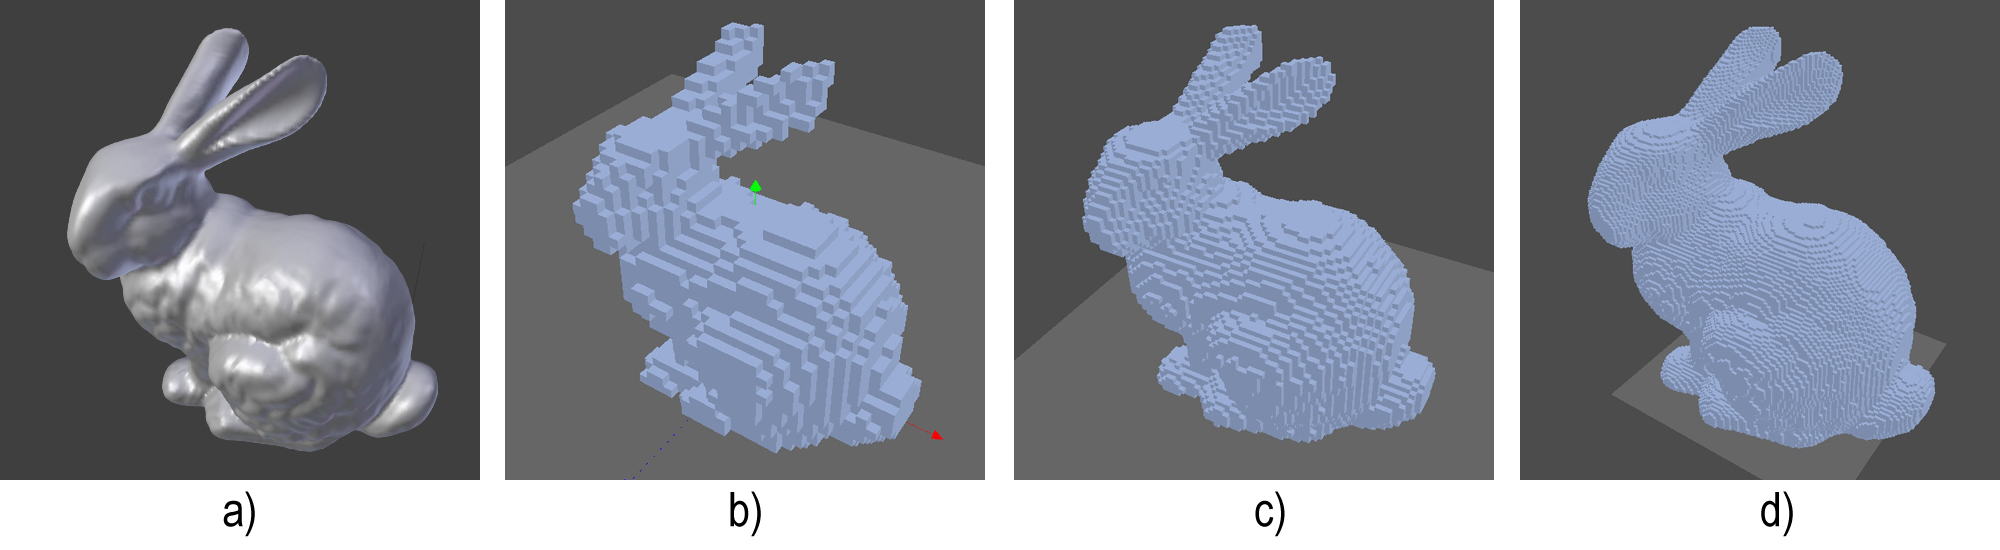
\includegraphics[width=1.0\textwidth]{bunny.jpg}
	\caption[Výsledky voxelizácie]{Výsledky voxelizácie. a) Originálny polygónový objekt b) $32^3$ c) $64^3$ d) $128^3$}
	\label{bunny}
\end{figure}

\section{Voxelové objekty}
Ako bolo spomenuté v kapitole \ref{chap:implementacia}, implementovali sme 5 základných voxelových tvarov: kváder, elipsoid, valec, ihlan a kužeľ. Výsledky implementácie môžete vidieť na obrázku \ref{shapes}. Na tomto obrázku vidno objekty v rozmeroch 20x20x20 voxelov, avšak je možné ich vytvoriť v ľubovoľných rozmeroch od 1 po 50. Aspoň takéto obmedzenia ponúka nami vytvorený interface na tvorbu voxelových tvarov.


Taktiež sme nad objektami implementovali boolovské operácie, ktoré v programe dosahovali očakávané výsledky ako je možné vidieť na obrázku \ref{bools}.


\begin{figure}[!h]
	\centering
	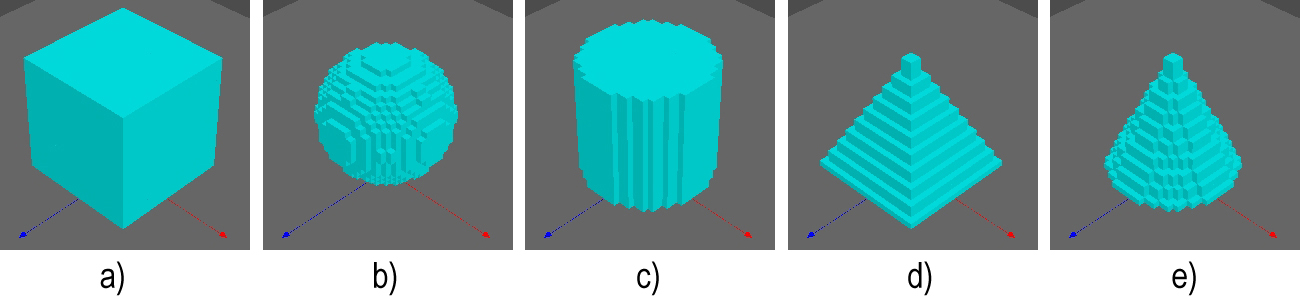
\includegraphics[width=1.0\textwidth]{shapes.jpg}
	\caption[Základné objekty]{Základné tvary. a) kocka(kváder) b) guľa(elipsoid) c) valec d) ihlan e) kužeľ }
	\label{shapes}
\end{figure}

\begin{figure}[!h]
	\centering
	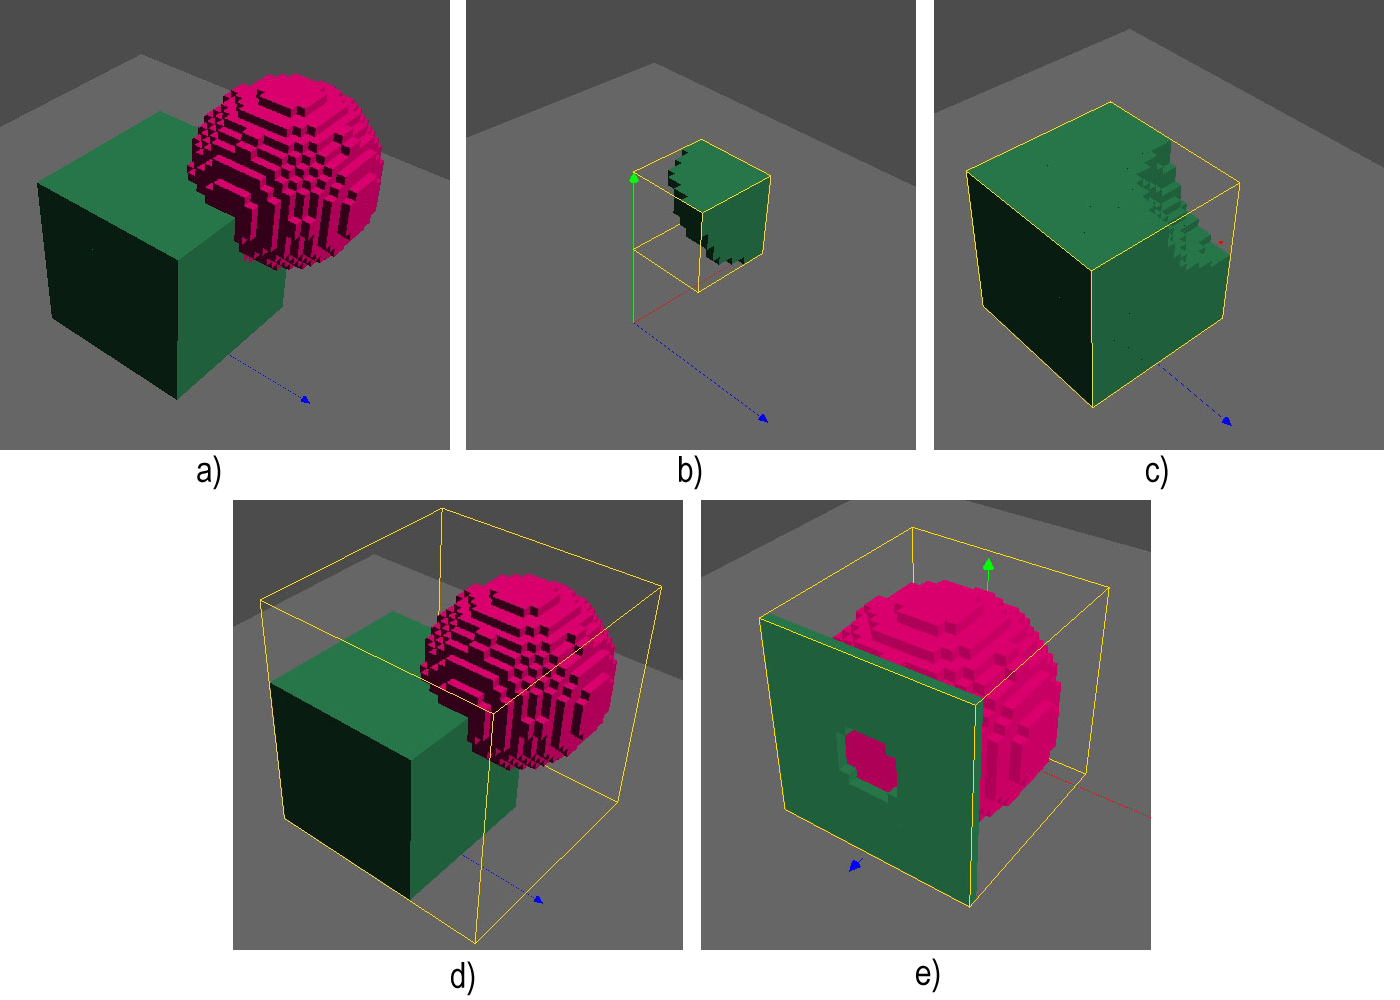
\includegraphics[width=1.0\textwidth]{bools.png}
	\caption[Booleanovské operácie]{Výsledok booleanovských operácií. a) Originálne objekty b) AND c) NOT d) OR e) XOR (nevznikol z objektov na obrazku a) )}
	\label{bools}
\end{figure}

\section{Nástroje}
Získavanie voxelov z objektu na kliknutie je dostatočne rýchle a teda základné nástroje, ktoré využívajú túto funkciu, ako napríklad \textit{štetec}, \textit{guma}, \textit{kvapkátko} a podobne, dosahujú želané výsledky a nestretli sme sa so žiadnymi závažnejšími problémami pri ich navrhovaní a ani používaní.

Zaujímavejším z nástrojov je napríklad nástroj \textit{výplň}, ktorého fungovanie je zložitejšie a časovo náročnejšie, keďže využíva algoritmus prehľadávania do šírky a teda v mnohých prípadoch prechádza cez všetky voxely objektu. Tento nástroj sme po prvotnom testovaní museli optimalizovať s použitím smerníkov, a tak sme dosiahli niekoľkonásobne väčšiu rýchlosť, keďže sme sa vyhli zbytočnému volaniu kopírovacích konštruktorov. 
 
Taktiež problémovými boli modifikačné nástroje s výnimkou translácie. V prípade škálovania a rotácie bolo potrebné vyriešiť vznikajúce diery, čo sa nám podarilo na základe spomenutých algoritmov v kapitole \ref{chap:implementacia} \textit{Implementácia} v sekcii \ref{voxelObjects} \textit{Voxelové objekty}. Výsledky našej implementácie týchto postupov môžete vidieť na obrázku \ref{modif}.
\begin{figure}[ht!]
	\centering
	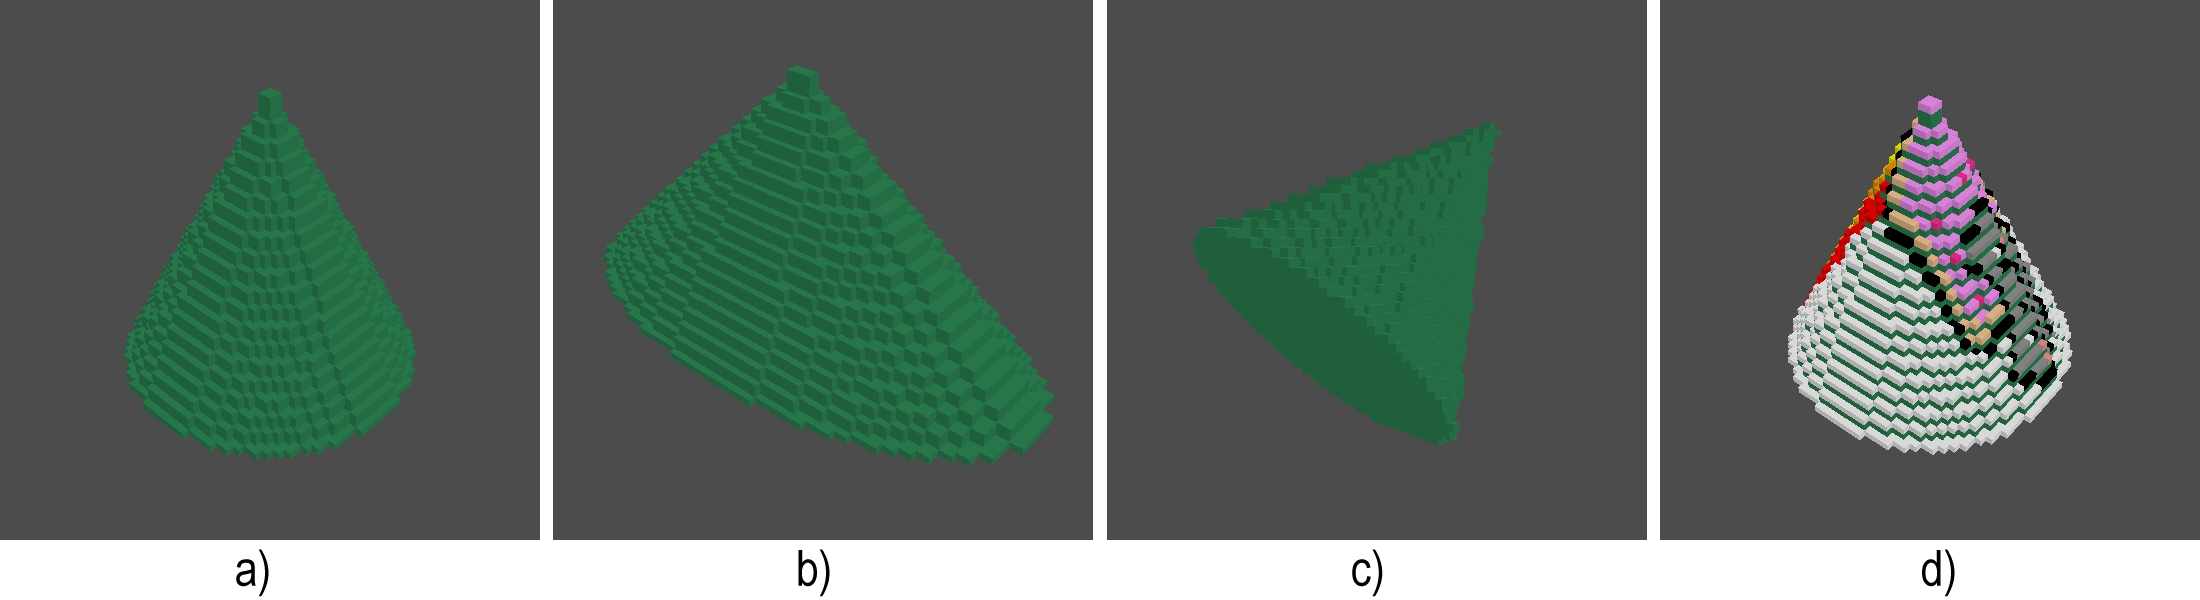
\includegraphics[width=1.0\textwidth]{modif.jpg}
	\caption[Transformácie obejktov]{Transformácie obejktov a textúrovanie. a) Pôvodný objekt  b) Naškálovaný objekt na dvojnásobnú šírku  c) Zrotovaný objekt o $45\,^{\circ}$ okolo osi $x$  d) Objekt s namapovanou textúrou}
	\label{modif}
\end{figure}

\section{Import/Export}
Testovanie importu a exportu voxelových súborov sme realizovali prostredníctvom programu na zobrazovanie voxelových objektov \textit{viewvox} a programu na voxelizáciu 3D modelov \textit{binvox} \cite{binvox}. Oba programy nepodporujú všetky nami implementované súborové formáty, preto bolo môžné vyskúšať ukladanie scény do formátov: .binvox, .mira a loadovanie súborov vygenerovaných programom binvox: .binvox, .mira, .vtk. 

Ako možno vidieť na obrázku \ref{io}, program viewvox pri zobrazovaní naškáluje objekt na rozmery $1\times1\times1$, čo spôsobuje deformáciu objektov, ktoré nemajú totožné všetky tri dimenzie. Ďalším rozdielom pri zobrazovaní je umiestnenie osí \textit{z} a \textit{y}, ktoré sú v našom prípade vymenené.

Pomocou programu binvox sme voxelizovali trojrozmerný polygónový objekt na voxelový o rozmeroch $64^3$ a uložili vo vyššie spomenutých formátoch. Takéto súbory sme sa potom snažili načítať do nášho prostredia. Prvý pokus nebol úspešný, ale po malých úpravách kódu sa nám súbory podarilo korektne spracovať a voxelové objekty načítať s vymenenou osou \textit{z} podobne ako pri programe viewvox. Ako bolo spomenuté v kapitole \ref{chap:implementacia} v sekcii \ref{sec:io} a ako možno vidieť na obrázku \ref{io} tieto formáty neumožňujú ukladanie farieb, a tak sa zobrazujú v defaultnej bielej farbe. 

Uskutočnili sme aj testy exportu a importu pre XML štruktúru. Výsledky boli očakávané a ničím zaujímavé, a preto ich tu ani neuvádzame.

\begin{figure}[!h]
	\centering
	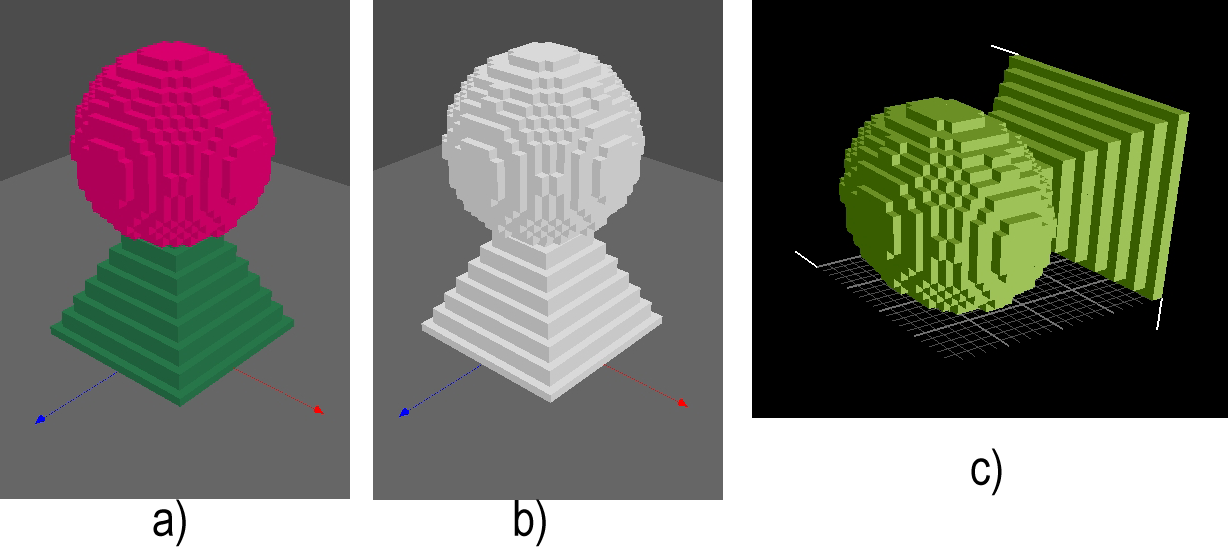
\includegraphics[width=0.8\textwidth]{export.png}
	\caption[Test exportu]{Výsledky testovania exportu do binárnych súborov. a) Exportovaný objekt b) Načítaný objekt v našom prostredí c) Načítaný objekt v programe viewvox}
	\label{io}
\end{figure}
\eject

Okrem importu meshu, teda voxelizácie, ktorej výsledky sme vyhodnotili vyššie, je možné do programu importovať rôzne obrázkové súbory.
 
Import bitmapy do prostredia bol taktiež zaujímavý. Podarilo sa nám vložiť akýkoľvek obrázkový formát, ktorý je schopná otvoriť knižnica DevIL, s výnimkou formátov, ktoré majú indexované farby ako napríklad gif. Na obrázku \ref{obr:cat} možno vidieť bitmapu mačky vo formáte PNG s transparentnými pixelmi (na obrázku ich vidno ako šedé) o rozmeroch $50\times50$ pixelov a objekt, ktorý vznikol importovaním tohoto obrázka do programu. Program zachováva transparenciu pixelov, ktoré majú hodnotu \textit{alpha} nulovú.

\begin{figure}[!h]
	\centering
	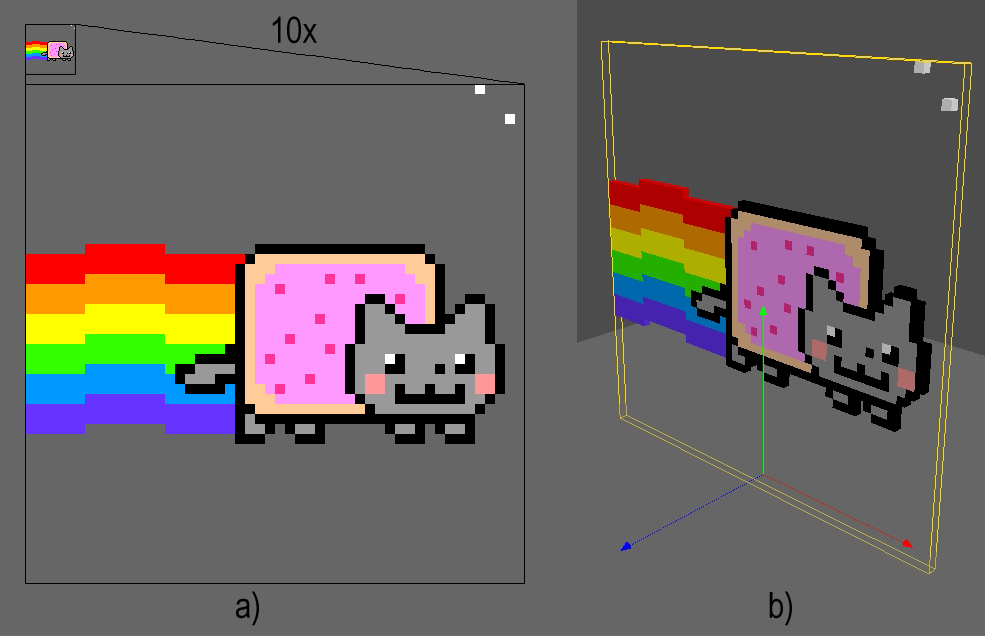
\includegraphics[width=0.8\textwidth]{cat.png}
	\caption[Import bitmapy]{Výsledok importu bitmapy. a) 10 násobne zväčšená bitmapa mačky b) importovaná bitmapa do prostredia}
	\label{obr:cat}
\end{figure}

\section{Užívateľské prostredie}
Pri tvorbe užívateľského prostredia sme kládli dôraz na vytvorenie čo najväčšieho pracovného priestoru. Výsledkom je, že najrozmernejšia časť okna aplikácie zaberá takzvané plátno, na ktoré je premietaná voxelová scéna. 

V ľavom paneli sa nachádzajú dve série ikoniek predelené oddeľovačom, z ktorých prvá sú základné editačné nástroje a druhá séria sú základné tvary, ktoré možno do prostredia vložiť. 

Ďalej sa tu nachádzajú ešte dve horizontálne lišty zarovnané na vrchný okraj okna. V jednej sa nachádzajú štyri ikonky, ktoré slúžia na booleanovské operácie nad objektami a druhá lišta obsahuje zvyšnú funkcionalitu programu, teda import a export, možnosť prepínania zobrazenia podlahy, osí, tieňovania a podobne a taktiež možnosť transformácie označených objektov.

Na obrázku \ref{ui} možno vidieť výsledné prostredie nášho editora, tak ako sme ho opísali v tejto sekcii.\\
\begin{figure}[!h]
	\centering
	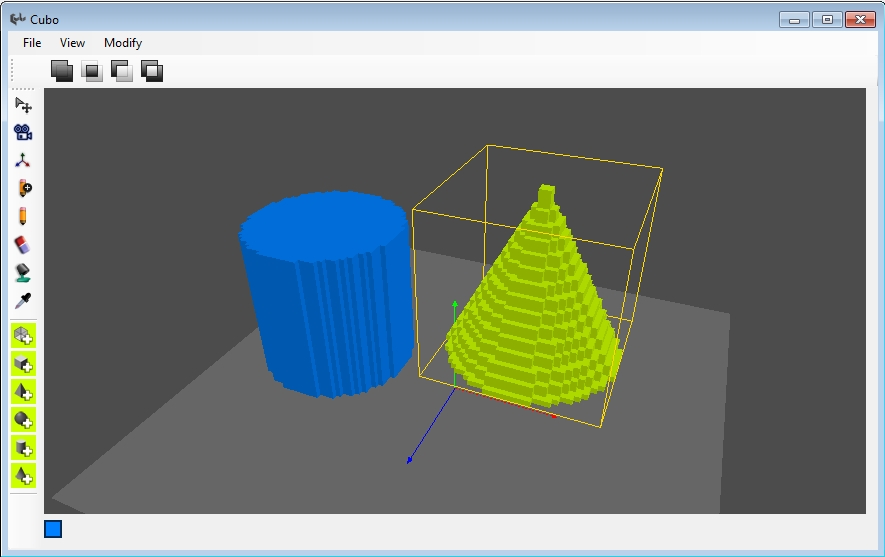
\includegraphics[width=1.0\textwidth]{UI.jpg}
	\caption[Užívateľské prostredie]{Screenshot z programu \textit{Cubo}}
	%\vspace*{3in}
	\label{ui}
\end{figure}